\documentclass[a4paper, 11pt]{article}
% ukazi za delo s slovenscino -- izberi kodiranje, ki ti ustreza
\usepackage[slovene]{babel}
\usepackage[utf8]{inputenc}
\usepackage[T1]{fontenc}
\usepackage[utf8]{inputenc}
\usepackage{amsmath,amssymb,amsfonts}
\usepackage{url}
\usepackage[normalem]{ulem}
\usepackage[dvipsnames,usenames]{color}
\usepackage{graphicx}
\usepackage{float}
\usepackage{verbatim}
\graphicspath{ {./slike/} }


% ukazi za matematicna okolja
%\theoremstyle{definition} % tekst napisan pokoncno
%\newtheorem{definicija}{Definicija}[section]
%\newtheorem{primer}[definicija]{Primer}
%\newtheorem{opomba}[definicija]{Opomba}

%\renewcommand\endprimer{\hfill$\diamondsuit$}


%\theoremstyle{plain} % tekst napisan posevno
%\newtheorem{lema}[definicija]{Lema}
%\newtheorem{izrek}[definicija]{Izrek}
%\newtheorem{trditev}[definicija]{Trditev}
%\newtheorem{posledica}[definicija]{Posledica}


% za stevilske mnozice uporabi naslednje simbole
\newcommand{\R}{\mathbb R}
\newcommand{\N}{\mathbb N}
\newcommand{\Z}{\mathbb Z}
\newcommand{\C}{\mathbb C}
\newcommand{\Q}{\mathbb Q}

% ukaz za slovarsko geslo
\newlength{\odstavek}
\setlength{\odstavek}{\parindent}
\newcommand{\geslo}[2]{\noindent\textbf{#1}\hspace*{3mm}\hangindent=\parindent\hangafter=1 #2}

% naslednje ukaze ustrezno popravi
\newcommand{\program}{Finančna matematika 1.~stopnja} % ime studijskega programa: Matematika/Finan"cna matematika
\newcommand{\imeavtorja}{Patrik Gregorič, Petja Murnik} % ime avtorja
\newcommand{\naslovdela}{Consecutive square packing}
\newcommand{\letnica}{2022} 
\newcommand{\predmet}{Finančni praktikum}

% vstavi svoje definicije ...

%%%%%%%%%%%%%%%%%%%%%%%%%%%%%%%%%%%%%%%%%%%%%%%


\begin{document}

\thispagestyle{empty}
\begin{center}
\begin{minipage}{0.75\linewidth}
    \centering
    {\Large Univerza v Ljubljani \\ \program}
    \\
    \vspace{3cm}

    {\uppercase{\Large \textbf{\naslovdela}}} \\ \predmet\\
    \vspace{3cm}

    {\Large \imeavtorja\par}
    \vspace{9cm}

\end{minipage}
\end{center}

\noindent{\large
Ljubljana, \letnica}
\pagebreak

\thispagestyle{empty}
\tableofcontents
\pagebreak


\section{Opis problema}

\subsection{Osnovni problem}
Za vsak celo število $i =1, \dots , n$ imamo en kvadrat s stranicami 
dolžine $i$. Želimo najti kvadrat z najkrajšo stranico, v katerega lahko 
zložimo vse kvadrate, ne da bi se notranjosti kvadratov prikrivale (robovi se lahko 
dotikajo). Kvadratov ne moremo obračati lahko jih samo transliramo.

\subsection{Ideja za reševanje}
Problem je enostavno predstavljiv. Imamo zaporedje vse večjih kvadratov, ki jih razporedimo
v ravnino, te se ne prekrivajo, se lahko dotikajo. Kvadratov ne smemo rotirati, lahko
jih le premikamo levo, desno, gor, dol. Omejila sva problem le na pozitivne $x$ in $y$
zaradi lažje predstave. Za majhen $n$ si je problem lahko predstavljati, saj ga
rešimo zelo hitro kar sami.

\begin{figure}[H]
    \centering
    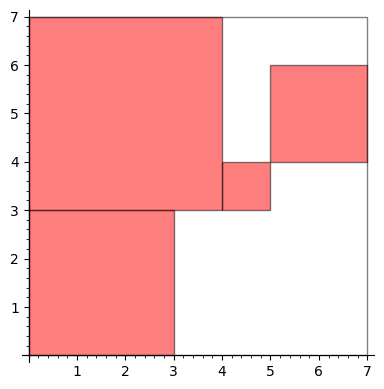
\includegraphics{prvi.png}
    \caption{Lahek primer za $n = 4$}
\end{figure}

Opazimo, da postavimo največja kvadrata drug zraven drugega in ostale le razporedimo s kar
veliko možnostmi na prosta mesta. Problem je enostaven, ker je veliko različnih možnosti.

\section{Reševanje osnovnega problema}
\subsection{Kratek opis}
Za večji $n$ postane problem mnogo težji. Zato sva se odločila reševati s celoštevilskim linearnim programiranjem.
To je: uvedla bova spremenljivke, zapisala omejitve in to poslala skozi vgrajene 
metode za reševanje CLP v programskem jeziku Sage.
\subsection{Potek reševanja}
Za podatke imava podane kvadrate s stranicami dolžine $i$, kjer $i = 1, \dots , n$, in $ i \in \Z, n \in \N$.
Ciljna funkcija najinega problema je iskanje $\min z$, kjer je $z$ dolžina stranice največjega kvadrata, v katerega
se zloži vse manjše kvadrate s stranicami $i = 1, \dots , n$.\\
Za reševanje problema sva definirala razred Kvadrat.
\begin{verbatim}
from sage.plot.polygon import polygon
class Kvadrat:

    def __init__(self, x, y, dolzina_stranice):
        self.x = x
        self.y = y
        self.dolzina_stranice = dolzina_stranice

    def narisi(self, barva="red"):
        return polygon(
            [(self.x, self.y), (self.x + self.dolzina_stranice, self.y),
             (self.x + self.dolzina_stranice, self.y + self.dolzina_stranice),
             (self.x , self.y + self.dolzina_stranice )],
            color=barva,
            edgecolor='black',
            alpha=0.5,
            zorder=2)

def narisi_rezultat_P(rezultat):
    k = Kvadrat(0,0,rezultat[0])
    rezultat1 = list(rezultat[1])
    K = k.narisi()
    pomoc = []
    for i in rezultat1:
        j = Kvadrat(i[0],i[1],i[2])
        pomoc.append(j)
    RISI = [K]
    for l in pomoc:
        m = l.narisi()
        RISI.append(m)
    show(sum(RISI[i] for i in range(len(RISI))))
\end{verbatim}
Tu sva definirala kvadrat kot levo krajišče $(x,y)$ in dolžino stranice. Drugi dve funkciji
\texttt{narisi} in \verb|narisi_rezultat_P| nam omogočata prikaz rezultatov, ki jih dobiva v obliki seznama.

\begin{verbatim}
def packing(kvadrati): #kvadrati je seznam cifer 
    p = MixedIntegerLinearProgram(maximization=False)
    x = p.new_variable()
    y = p.new_variable()
    zg_meja = sum(kvadrati) + 1
    a = p.new_variable(binary = True) #kvadrat i ni levo od j
    b = p.new_variable(binary = True) #kvadrat j ni desno od j
    p.set_objective(p['z'])
    p.add_constraint((p['z']) >= (max(kvadrati)))
    for i, d in enumerate(kvadrati): # i je indeks, d je dolžina stranice
        p.add_constraint(x[i] >= 0)  # želimo nenegativne koordinate
        p.add_constraint(y[i] >= 0)
        p.add_constraint(x[i] + d <= p['z']) # omejimo p['z'] z največjo pokrito koordinato
        p.add_constraint(y[i] + d <= p['z'])
        for j , g in enumerate(kvadrati):
            p.add_constraint(x[i] + d <= x[j] + zg_meja * a[i,j])
            p.add_constraint(x[j] + g <= x[i] + zg_meja * a[j,i])
            p.add_constraint(y[i] + d <= y[j] + zg_meja * b[i,j])
            p.add_constraint(y[j] + g <= y[i] + zg_meja * b[j,i])           
    for i, j in Combinations(range(len(kvadrati)), 2):
        p.add_constraint(a[i, j] + a[j, i] + b[i, j] + b[j, i] <= 3)
    z = p.solve()
    xx = p.get_values(x)
    yy = p.get_values(y)
    return (z, [(xx[i], yy[i], d) for i, d in enumerate(kvadrati)])
\end{verbatim}

\noindent Ta CLP nam reši problem tudi za večji $n$, do katere rešitve ne pridemo tako intuitivno. Funkcija 
sprejme seznam cifer v obliki $range(1, n +1)$ in vrne $tuple$, ki vsebuje za prvi element dolžino
največjega kvadrata, torej rešitev problema, naslednji element je pa seznam kvadratov, ki so podani od
največjega do najmanjšega. Program najprej preveri, da so vse koordinate nenegativne, saj sva tako definirala
problem. Nato preverimo pogoje, da morajo biti vsi kvadrati znotraj največjega, ki ga želimo minimizirat in še, da 
se noben od njih ne sme prekrivat. S pomočjo teh omejitev nam program poda pravilno rešitev, ki jo nato še prikaževa s
funkcijo \verb|narisi_rezultat_P|.

\begin{figure}[H]
    \centering
    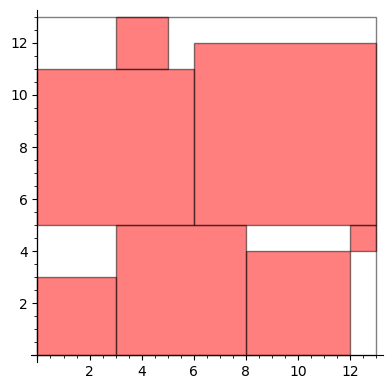
\includegraphics{Lahek_primer.png}
    \caption{Primer za $n = 7$}
\end{figure}

\noindent Opazimo, da problem hitro postane bolj kompleksen za reševanje.

\section{Nadgradnja problema}
\subsection{Opis nadgradnje}
V nadeljevanju bova problem tudi reševala v primeru, 
če namesto enega kvadrata z dolžino 
stranice vzamemo dva/tri/štiri \dots take kvadrate. 
Obravnavala bova tudi primer, ko je lahko ena točka v ravnini (velikem kvadratu) pokrita z 
dvema/tremi/štirimi \dots  kvadrati.



\end{document}